\documentclass[a4paper, 10pt]{article}
\usepackage[UTF8]{ctex}
\usepackage{geometry}
\geometry{left=3cm,right=3cm,top=3cm,bottom=3cm}
\usepackage{subfigure}
\usepackage[graphicx]{realboxes}
\begin{document}
  \title{\textbf{实验报告:测量介质中的声速}}
  \author{郑志恒 2300012559}
  \maketitle
\section{数据记录、处理与分析}
\subsection{共振频率的测量结果}
\vspace{10pt}
\begin{center}
\begin{tabular}{|c|c|c|c|c|c|}
    \hline
    i&1&2&3&4&5\\
    \hline
    f(kHz)&38.0&38.1&37.8&37.8&37.8\\
    \hline
    Upp(V)&5.0&8.0&4.0&6.0&3.0\\
    \hline
\end{tabular}
\end{center}
\vspace{10pt}

\noindent 测得共振频率为37.8kHz(此时室温24.1°C)。

\subsection{驻波法测量声速}
\begin{center}
    \begin{tabular}{|c|c|c|c|c|c|c|c|c|c|c|}
        \hline
        i&1&2&3&4&5&6&7&8&9&10\\
        \hline
        $x_i(mm)$&22.849&27.517&32.170&36.865&41.419&46.120&50.755&55.399&59.995&64.680\\
        \hline
        Upp(V)&1.19&0.856&0.696&0.512&0.401&0.365&0.340&0.304&0.268&0.236\\
        \hline
        $x_i^*(mm)$&64.665&59.980&55.380&50.743&46.118&41.450&36.825&32.149&27.525&22.850\\
        \hline
        Upp(V)&0.240&0.266&0.298&0.340&0.360&0.408&0.512&0.692&0.844&1.21\\
        \hline
    \end{tabular}
    \end{center}

\subsubsection{逐差法处理数据}
\noindent (i)增大时:
$$\Delta x_1=x_6-x_1=23.271$$
$$\Delta x_2=x_7-x_2=23.238$$
$$\Delta x_3=x_8-x_3=23.229$$
$$\Delta x_4=x_9-x_4=23.130$$
$$\Delta x_5=x_{10}-x_5=23.261$$
有:
$$\Delta \overline{x}=23.2258$$
测得波长有:
$$\lambda_1=\frac{2}{5}\Delta \overline{x}=9.290mm$$
不确定度有:
$$\sigma_{\Delta \overline{x}}=\sqrt{\frac{1}{n-1}\sum_{i=1}^n(\Delta x_i-\Delta \overline{x})^2}=0.056$$
坏值检验:
$$3\sigma_{\Delta \overline{x}}=0.19$$
故该测量没有坏值。

\noindent A类不确定度:
$$\sigma_a=\frac{\sigma_{\Delta \overline{x}}}{\sqrt{n}}=0.025mm$$
B类不确定度:
$$\sigma_b=\frac{e}{\sqrt{3}}=0.0023mm$$

\noindent 故总的不确定度为:
$$\sigma=\frac{2}{5}\sqrt{\sigma_a^2+\sigma_b^2}=0.01mm$$

\noindent (ii)减小时:
$$\Delta x_1=x_6-x_1=-23.215$$
$$\Delta x_2=x_7-x_2=-23.155$$
$$\Delta x_3=x_8-x_3=-23.231$$
$$\Delta x_4=x_9-x_4=-23.218$$
$$\Delta x_5=x_{10}-x_5=-23.268$$
有:
$$\Delta \overline{x}=23.2174$$
测得波长有:
$$\lambda_2=\frac{2}{5}\Delta \overline{x}=9.287mm$$
不确定度有:
$$\sigma_{\Delta \overline{x}}=\sqrt{\frac{1}{n-1}\sum_{i=1}^n(\Delta x_i-\Delta \overline{x})^2}=0.041$$
坏值检验:
$$3\sigma_{\Delta \overline{x}}=0.12$$
故该测量没有坏值。

\noindent A类不确定度:
$$\sigma_a=\frac{\sigma_{\Delta \overline{x}}}{\sqrt{n}}=0.018mm$$
B类不确定度:
$$\sigma_b=\frac{e}{\sqrt{3}}=0.0023mm$$

\noindent 故总的不确定度为:
$$\sigma=\frac{2}{5}\sqrt{\sigma_a^2+\sigma_b^2}=0.007mm$$

\noindent 因此,总的波长测量值和不确定度为:

$$\lambda=(\lambda_1+\lambda_2)/2=9.289mm$$

$$\sigma=0.012mm$$
波长测量结果表达式为:
$$\lambda=(9.29\pm0.012)mm$$

\noindent 利用公式$v=\lambda f$计算波速得到$v=351.16m/s$,假设信号发生器的误差不超过0.5\%,即$\sigma_f=0.189kHz$,可以得到$\sigma_v=\sqrt{(f\sigma)^2+(\sigma_f \lambda)^2}=1.813m/s$。综上,速度的测量结果为$v=(351\pm1.8)m/s$

\subsection{相位法测量声速}
\begin{center}
    \begin{tabular}{|c|c|c|c|c|c|c|c|c|c|c|}
        \hline
        i&1&2&3&4&5&6&7&8&9&10\\
        \hline
        $x_i(mm)$&25.215&34.470&43.801&53.029&62.325&71.745&81.008&90.250&99.578&108.823\\
        \hline
        
        $x_i^*(mm)$&108.529&99.890&90.233&80.820&71.619&62.350&53.025&43.798&34.495&25.210\\
        \hline
        
    \end{tabular}
    \end{center}
\subsubsection{最小二乘法处理数据}
\noindent (i)增大时:
$$\sigma_{x}=e/\sqrt{3}=0.0023mm$$
\noindent 斜率的不确定度:
$$\sigma_{k}=\sqrt{(\sigma_{ka})^2+(\sigma_{kb})^2}=0.0027mm$$
波长的计算结果为:
$$\lambda_1=9.290mm$$
\noindent (ii)减小时:
$$\sigma_{x}=e/\sqrt{3}=0.0023mm$$
\noindent 斜率的不确定度:
$$\sigma_{k}=\sqrt{(\sigma_{ka})^2+(\sigma_{kb})^2}=0.0028mm$$
波长的计算结果为:
$$\lambda_1=9.258mm$$
综上,最小二乘法的测量结果为:$\lambda=(9.274\pm0.0039)mm$

\noindent 利用公式$v=\lambda f$计算波速得到$v=350.55m/s$,假设信号发生器的误差不超过0.5\%,即$\sigma_f=0.189kHz$,可以得到$\sigma_v=\sqrt{(f\sigma)^2+(\sigma_f \lambda)^2}=1.759m/s$。综上,速度的测量结果为$v=(351\pm1.8)m/s$
    \subsection{气体状态法测量声速}
\vspace{10pt}
    \begin{center}
        \begin{tabular}{|c|c|c|c|}
            \hline
            t/°C&P/Pa&H&Ps/Pa\\
            \hline
            24.1& $1.023\times 10^5$&42\%&2337.8\\
            \hline
    
        \end{tabular}
        \end{center}

$$v=331.45\sqrt{(1+\frac{t}{T})(1+\frac{0.3192Ps}{P})}=347.02m/s$$
其中:
$$\sigma_t=0.189k$$
$$\sigma Pw=\sigma P=0.01Pa$$
$$\sigma\approx 0.06m/s$$
因此气体状态法的测量结果为:
$$v=(347.02\pm0.06)m/s$$

\subsubsection{声波振幅随距离衰减图}
\begin{figure}[ht]
    \centering 
    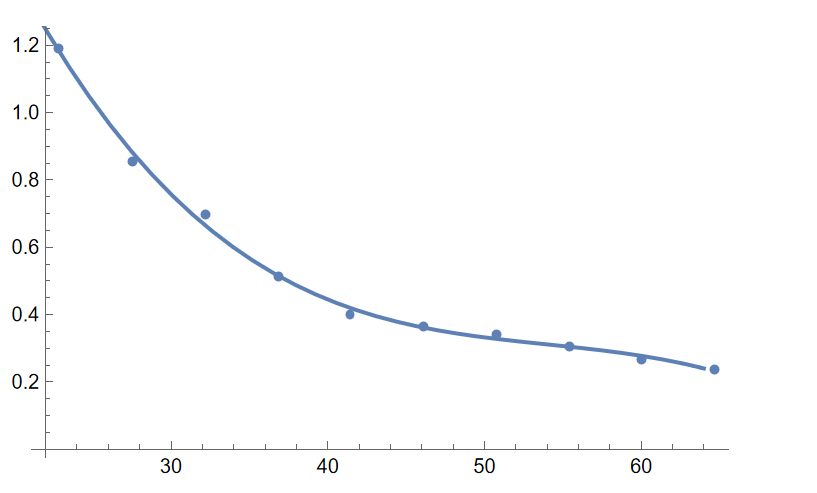
\includegraphics[height=5.5cm,width=9.3cm]{pic1.png}
    
    \caption{多项式拟合}
    \label{3}
    
    \end{figure}
\noindent 前一段用二次函数拟合较为贴近,猜测声波振幅随距离增大而平方反比衰减。

\section{实验讨论}
\noindent \textbf{误差评价:}

\vspace{10pt}
\noindent 1.在极值法测量时,我发现很难找到一个长度使得峰值稳定在最大值。峰峰电压总是处于不停地振动中,因此最大峰峰电压对应的x的值也在变化,我认为现有的对误差的评价并没有包含该因素,且我认为这属于随机误差。

\vspace{10pt}
\noindent 2.在气体状态法测量声速时,测量结果与前两种方法测得的值差距过大(即使算上误差),我认为这是由于我使用的温度是手机APP记录的当地室外天气,这使得该温度与实验室中的温度存在一定区别。(且该公式本身可能并不严格)

\vspace{10pt}
\noindent 3.在观察李撒如图形时,有时为了使李撒如图形稳定在最精准的直线图形,我需要不断朝不同的方向转动螺母。因此,我认为这其中可能仍旧存在一部分回程差没有被计入。

\vspace{10pt}
\noindent \textbf{相位法和极值法的比较:}
\vspace{10pt}

\noindent 相位法比极值法更准。误差主要来源于:
\vspace{10pt}

\noindent 1.在简谐运动的测量中,测量最大变化率点往往比测量最大值点更准
\vspace{10pt}

\noindent 2.驻波法(极值法)的测量结果受次峰的影响比较明显,而相位比较法基本不受次峰的影响。次峰的出现可能会使得极值点的位置不准确,从而影响波长的测量和最终的声速计算

\noindent \textbf{频率、距离、声压是否对声速有影响(补充实验):}

\vspace{10pt}
\noindent 我选择的是频率对声速的影响,记录了在振幅为100\%,50\%,25\%,10\%时候对应频率和此时的声速。实验数据如下:

\begin{center}
    \begin{tabular}{|c|c|c|c|c|c|c|}
        \hline
        100\%(f=38.542kHz)&1&2&3&4&5&6\\
        \hline
        $x_i(mm)$&23.693&27.240&31.840&36.405&40.987&45.515\\
        \hline
        
        
        
    \end{tabular}
    \end{center}
    \begin{center}
        \begin{tabular}{|c|c|c|c|c|c|c|}
            \hline
            50\%(f=38.631kHz)&1&2&3&4&5&6\\
            \hline
            $x_i(mm)$&22.680&27.215&31.793&36.337&40.950&45.440\\
            \hline
            
            
            
        \end{tabular}
        \end{center}
        \begin{center}
            \begin{tabular}{|c|c|c|c|c|c|c|}
                \hline
                25\%(f=39.364kHz)&1&2&3&4&5&6\\
                \hline
                $x_i(mm)$&22.480&26.955&31.422&35.938&40.382&44.847\\
                \hline
                
                
            \end{tabular}
            \end{center}
            \begin{center}
                \begin{tabular}{|c|c|c|c|c|c|c|c|c|c|c|}
                    \hline
                    25\%(f=40.174kHz)&1&2&3&4&5&6\\
                    \hline
                    $x_i(mm)$&22.318&26.690&31.095&35.490&39.910&44.182\\
                    \hline
                    
                \end{tabular}
                \end{center}
    测得不同频率下声速为:
    \begin{center}
        \begin{tabular}{|c|c|c|c|c|}
            \hline
            f(kHz)&38.542&38.631&39.364&40.174\\
            \hline
             v(m/s)&336.43&351.70&352.18&351.34\\
            \hline
            
        \end{tabular}
        \end{center}
结论:在非谐振频率下,即不是换能器的谐振频率时,测得的声速相对其他频率来说稍微偏大,这是由于非谐振频率下次级峰导致的误差较大。

\section{思考题}
\noindent 1.为什么不测量单个的$\lambda$/2或$\lambda$,而要测量多个?在计算$\lambda$/2或$\lambda$时,将所测数据首尾相减,再除以$\lambda$/2或$\lambda$的个数:这种计算方法与逐差法比较,哪一种较好?

\vspace{10pt}
\noindent 答:测量多个波长是为了减小随机误差。如果将所测数据首尾相减再除以波长个数,相当于只利用了两个测量数据,没有尽可能利用更多的测量数据减小实验误差。逐差法尽可能地利用了更多的测量数据,因此更能减小随机误差,从而减小不确定度,使得测量和计算的结果更准确。

\vspace{10pt}
\noindent 2.用第一种方法,为什么要在正弦波振幅为极大时进行测量?用第二种方法,为什么要在李萨如图形呈直线时进行测量?

\vspace{10pt}
\noindent 答:用极值法测量时,波腹出现时变化比较剧烈,此时进行测长,仪器的灵敏度较高,因此选择在振幅达到最大值时进行记录;使用李撒如图形进行测量时,也是因为直线图形的辨识度较高,更容易精准地判断波长达到整数间隔时的对应位置,从而使得测量更加准确。

\end{document}